%%% Local Variables: 
%%% mode: latex
%%% TeX-master: t
%%% End: 

\chapter{CMS事例模拟与重建}

\section{CMS事例模拟}

质子-质子对撞相比于正负电子对撞最大的优势就是对撞中心能量可以非常高,但是与此同时,质子-质子对撞也有明显的劣势:本底环境非常复杂。在电弱尺度下,发生对撞的主要是质子中的夸克和胶子,而质子内部含有非常多的胶子和夸克,这就使得对撞发生时会有非常多的本底,对我们所要寻找的物理过程产生严重阻挠。因此,理解对撞数据中的本底事例对最终的信号提取具有至关重要的作用。与此同时,除了扣除本底外,因为对撞事例中同时包含信号事例和本底事例,但是由于统计量的原因,信号事例被淹没在本底事例之中;或者对于新物理的寻找,我们不知道它具体出现在哪里。这时,可以通过对信号的模拟与数据做对比或者拟合,来得出信号在数据中的成分。因此,事例模拟在粒子物理实验中有着至关重要的作用。

目前,CMS实验通过使用基于蒙特卡洛(Monte Carlo, MC)方法的计算机模拟来对粒子物理实验中的各个本底事例和信号事例进行模拟。由于需要详尽的模拟对撞机中发生的物理过程,模拟一共分为两个阶段,分别为物理事例的产生模拟和事例在探测器中的模拟。

物理事例的产生模拟主要用来模拟每次对撞时发生的物理过程,包括最初的硬散射过程、强子化过程以及之后的非硬散射过程模拟(underlying Event, UE)。这些模拟可以通过不同的产生子来实现,比如:Madgraph~\cite{alwall2014automated},Herwig~\cite{bellm2016herwig},Pythia~\cite{sjostrand2008brief},Sherpa~\cite{gleisberg2009event},POWHEG~\cite{alioli2010general}。通过模拟我们可以得到产生子级别的事例信息,而后这些信息将用于模拟粒子在探测器中的响应。

探测器模拟主要用于模拟对撞产生的粒子在探测器中的响应,包括模拟事例在探测器中的运动轨迹、沉积能量以及与探测器物质发生相互作用后的情形等等。目前,CMS实验所使用的探测器模拟是基于GEANT4~\cite{agostinelli2003geant4}的软件框架,模拟包括了CMS探测器的所有子探测器以及构成探测器的其他成分。

\section{CMS事例重建}

在事例通过触发的选择后,存储下来的原始数据包含了粒子在各个子探测器中的响应,这些数据本身只是一些电子学信号,并不能够直接用于物理分析。但是,由于不同的粒子在整个探测器中留下的电子学信号不同,可以根据这些信号重建出最初的物理对象,比如:光子、电子、缪子和强子喷注,这种重建方法被称为粒子流算法(particle-flow algorithm, PF)。

如图~\ref{fig:c03f01}所示,粒子流算法的主要目的是结合各个子探测器的信息重建出对撞事例中的稳定粒子,比如电子、光子、缪子以及比较稳定的强子,算法优化了对粒子的种类、方向和能量的辨别。而后,这些稳定的粒子被用来重建更高阶的物理对象,比如喷注、$\tau$子、丢失的横向能量(missing transverse energy);也可以用来计算带电轻子或者光子的隔离度(isolation)等等。

\begin{figure}[!htbp]
    \centering
    %trim option's parameter order: left bottom right top
    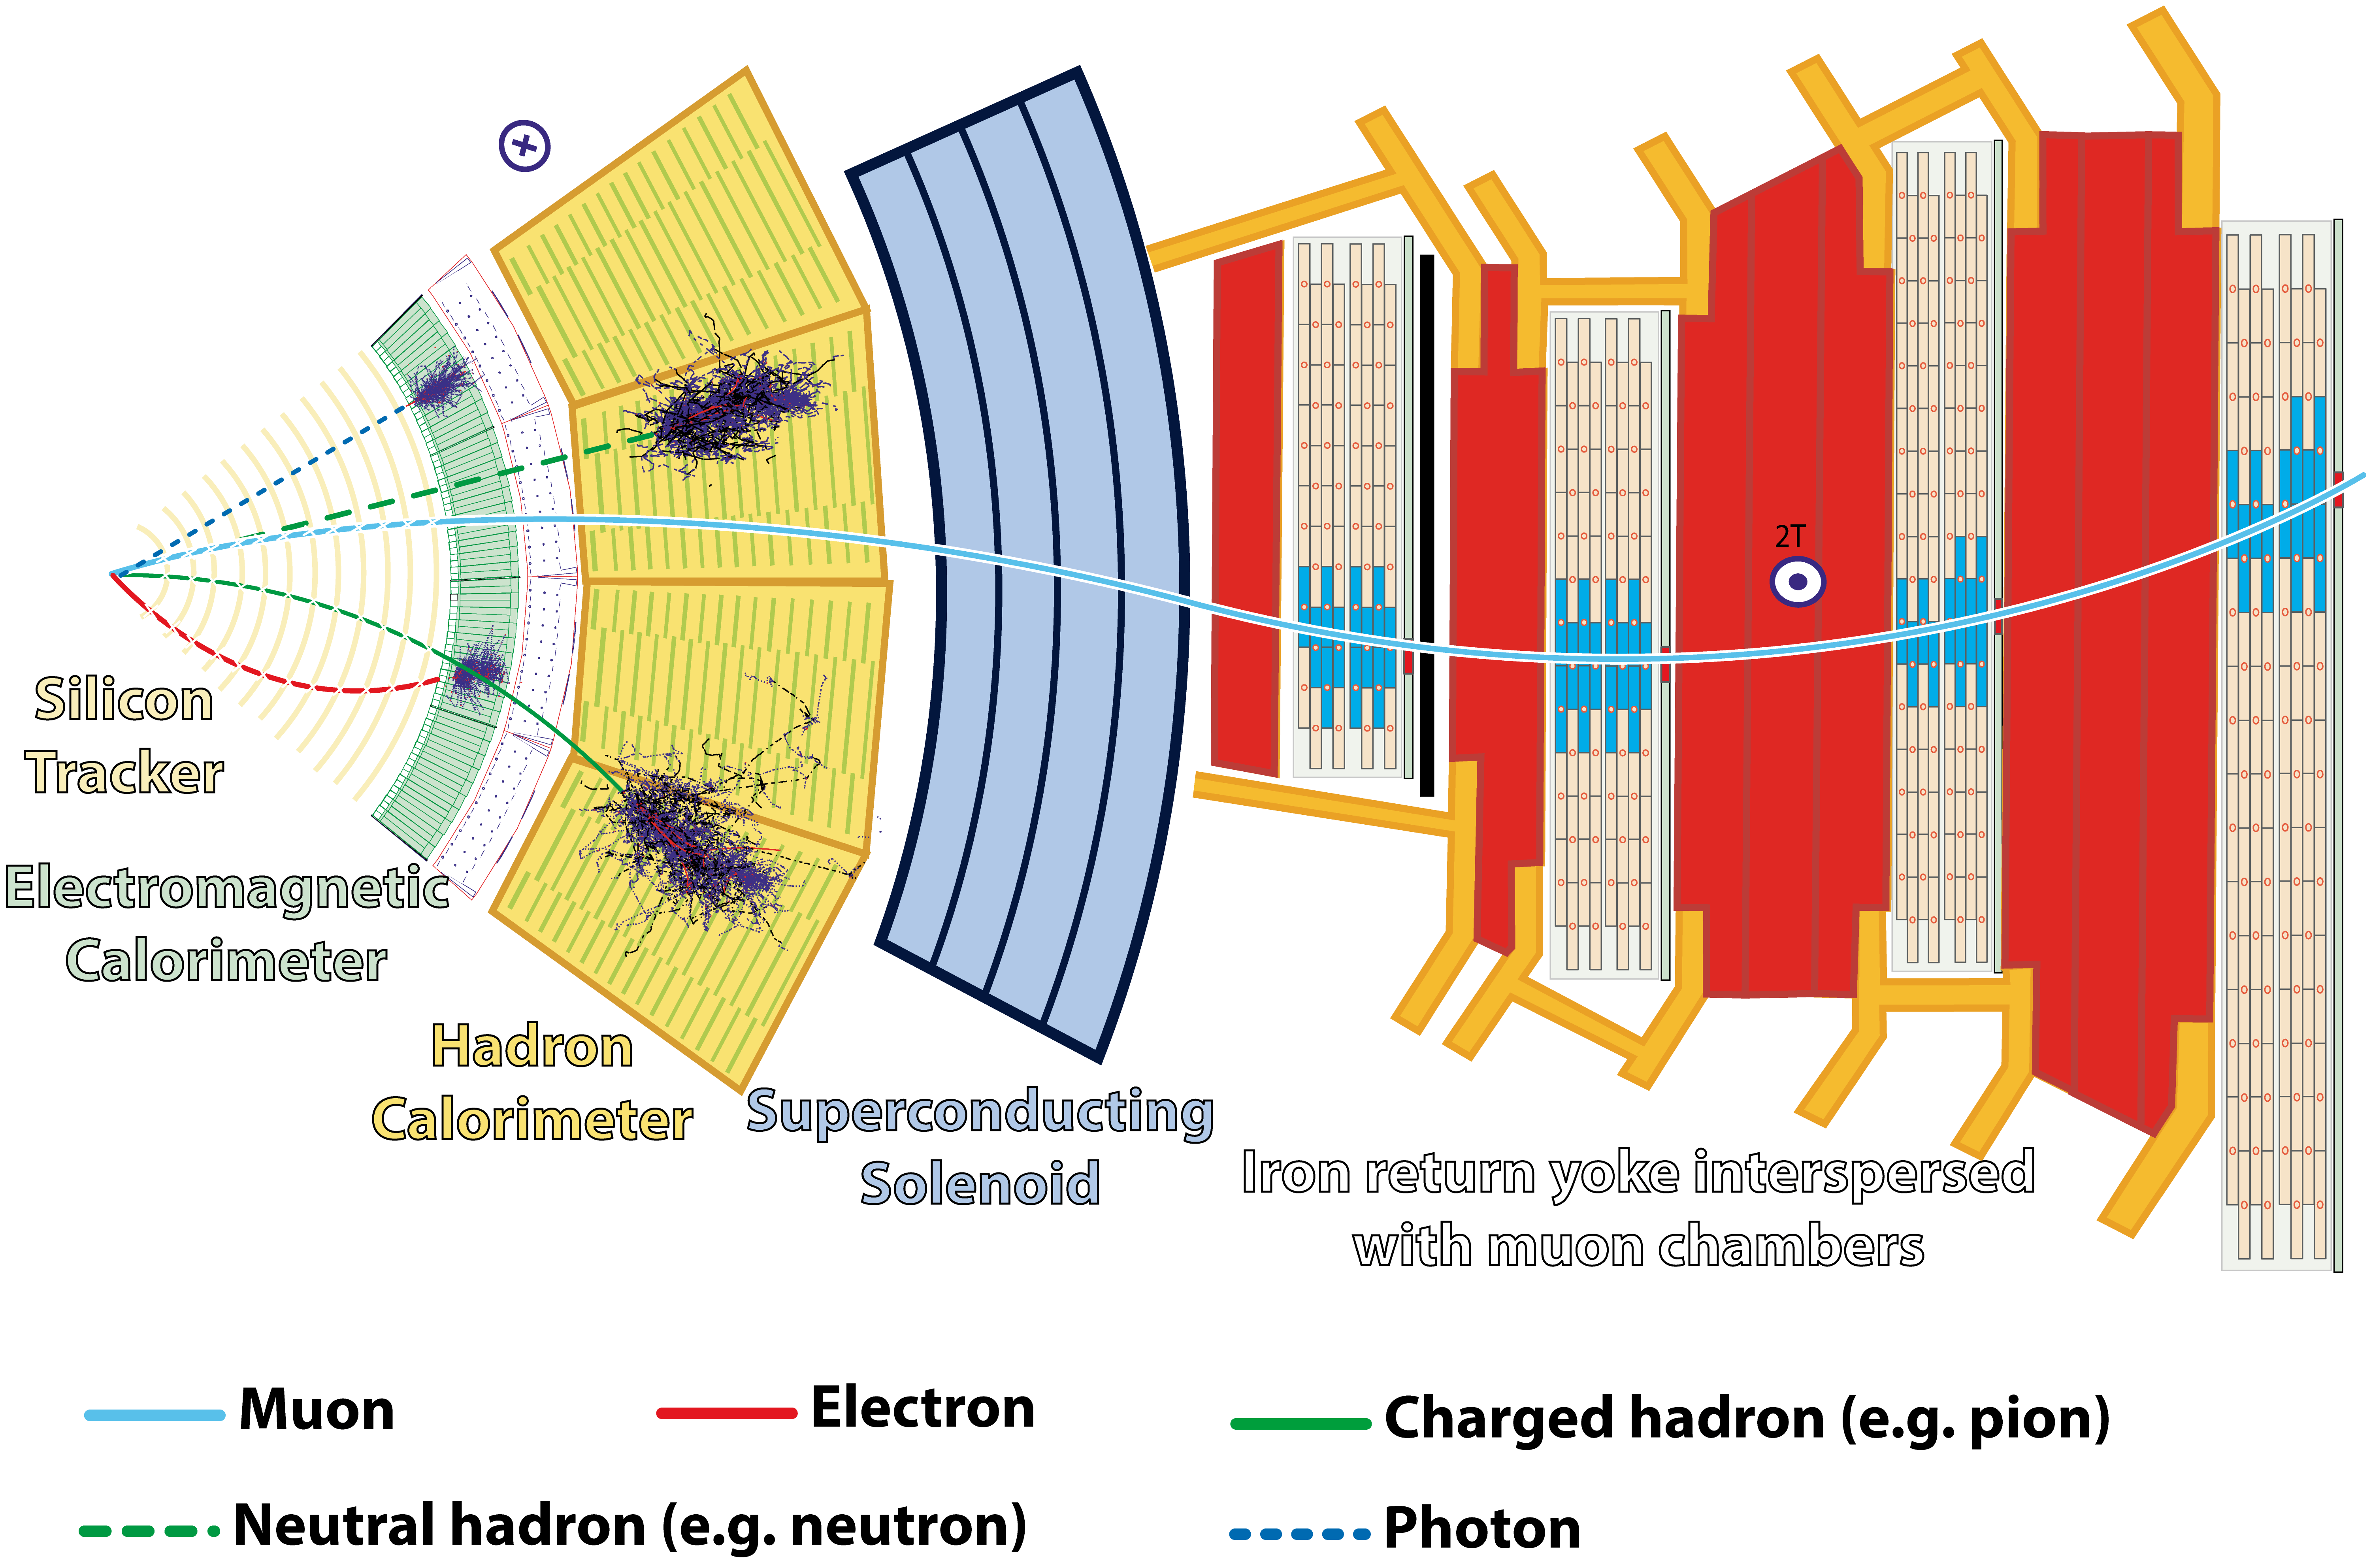
\includegraphics[width=0.6\textwidth]{figures/chapter03/CMSslice_whiteBackground.png}
    \bicaption{\quad \centering 不同粒子在探测器中的响应~\cite{Barney:2120661}}{\quad \centering Responses of different particles in the detector~\cite{Barney:2120661}}
    \label{fig:c03f01}
\end{figure}

粒子流算法重建事例的基本元素包括中心径迹探测器内重建出的对撞顶点和带电粒子的轨迹、电磁量能器和强子量能器中重建出来的能量簇射以及缪子探测器中重建出的缪子轨迹。带电粒子的轨迹是利用迭代跟踪的策略重建出来的,对于动量高达150$\GeV$的带电粒子,粒子流算法仍然可以同时保持非常高的效率和非常低的误判率。能量簇射是在各个量能器子探测器中利用专门的簇射算法构建出来的,这个算法是专为粒子流算法所设计,主要目的是为了可以对低能粒子和能量沉积相距比较近的粒子保持比较高的探测效率。而后,这些基本元素通过连接算法连接起来用于完整的重建出单个粒子,同时删除不同子探测器中可能出现的重复计数。

对于光子和电子的辨别,这两者在探测器中的响应非常相似,都可以被电磁量能器所吸收并测量其能量,而且这两者在电磁量能器中的簇射形状也十分类似,但是由于光子不带电荷而电子带电荷,使得电子可以在中心的径迹探测器内留下轨迹并且在磁场的作用下发生偏转,而光子不会在径迹探测器内留下轨迹。因此,粒子流算法通过辨别在电磁量能器中沉积能量的粒子是否同时在中心径迹探测器中留下轨迹来辨别出电子和光子。强子喷注主要是由对撞产生的夸克和胶子在探测器中的强子化过程所产生。对于带电的夸克产生的喷注会在径迹探测器中留下径迹并被磁场所弯曲,而中性强子或者胶子只会在强子量能器中产生簇射并被探测器所接收。由于缪子和其他物质的相互作用非常弱,它会穿过强子量能器到达外围的缪子探测器并在其中留下轨迹。粒子流算法可以通过缪子探测器以及中心径迹探测器中的信号来辨别缪子。当所有的物理对象重建出来后,一部分不可探测的粒子,比如中微子,会飞出探测器,但是根据横向动量守恒,我们可以根据其它所有物理对象重建出丢失的横动量。

\subsection{径迹室轨迹和对撞顶点重建}\label{subsec:PVReco}

CMS实验中,对中心径迹室中带电粒子运动轨迹的重建依赖于对撞产生的带电粒子穿过径迹探测器时所留下的击中信息。利用这些信息,可以通过使用基于组合卡尔曼滤波法(Combinatorial Kalman filter)的“迭代追踪”的方法重建出带电粒子的轨迹。这种方法首先对比较容易辨别的轨迹进行迭代重建,它们往往对应于横动量比较高、留下的击中信息比较完整的带电粒子轨迹。而后,将这些用于重建轨迹的击中排除,剩余的轨迹仅从剩下的击中中进行重建。这种方法可以有效降低轨迹重建时击中组合的复杂度,从而可以更好的对处于比较困难的动力学区域内的轨迹进行重建。轨迹重建的具体步骤可以分为以下四步:
\begin{itemize}
    \item 首先,对轨迹种子(Seed)进行重建,这一步对轨迹参数提供了初始估计值;
    \item 其次,将最初估计的候选轨迹传递到整个径迹室,利用卡尔曼滤波的方法找出每层探测器中与之对应的击中,并且对候选轨迹进行更新;
    \item 然后,将所有确定的击中进行合并拟合;
    \item 最后,选择质量较好的轨迹并进行保存,用于之后的物理对象重建。
\end{itemize}
目前,CMS实验中对径迹室内的带电粒子的轨迹重建效率在横动量大于1$\GeV$的条件下可以达到90\%左右~\cite{Elmetenawee:2020emw}。

由于在对撞过程中,会产生除了我们所关注的硬散射过程以外的其他过程,使得每次束流对撞都会产生数量众多的堆积事例(Pileup event),在探测器中心处可以同时观测到多个对撞顶点,而其中只有一个对撞顶点是我们所感兴趣的顶点。因此,对初级对撞顶点的重建和筛选对完整重建出我们所感兴趣的物理过程具有非常重要的物理意义。

目前,CMS实验中对撞顶点的重建主要利用了在径迹探测器中重建出来的带电粒子的轨迹,它可以对每个事例中质子质子相互作用顶点的位置和不确定度进行测量。对撞顶点的具体重建步骤可以分为以下三步:
\begin{itemize}
    \item 首先,对重建出来的轨迹进行挑选,要求选中的轨迹相对于束流点(Beam spot)的中心位置的横向对撞参数小于5、轨迹在硅像素探测器中至少含有两个击中、在硅像素和硅微条探测器中一共含有至少5个击中以及每条轨迹拟合所得到的归一化$\chi^{2}$值小于20;
    \item 然后,根据所有轨迹相对于束流点在$z$方向的最短距离对来自于同一对撞顶点的轨迹进行聚类;
    \item 最后,根据所有聚类后的轨迹拟合出对撞顶点。
\end{itemize}
这一方法可以对来自同一对撞的所有顶点进行重建,包括我们所感兴趣的硬散射过程初级顶点和堆积事例顶点。而对于初级对撞顶点的选择,CMS实验利用了重建顶点所对应的轨迹信息,选择硬散射程度最高的顶点作为初级对撞顶点。

\subsection{电子和光子的重建}\label{subsec:EGReco}

电子和光子的簇射会在电测量能器的几个晶体中沉积能量,大约94\%的能量可以沉积在3$\times$3的晶体块中,而5$\times$5的晶体块可以沉积大约97\%的能量。通过对沉积在这些晶体矩阵块中的能量进行求和,可以得出电子或光子的能量。但是由于电磁量能器内部其他物质的存在,使得电子会发生韧致辐射,光子会转换为正负电子对。在强磁场的作用下,到达量能器的能量会在$\phi$角度发散,对于这部分能量,CMS实验采取了超聚类算法(super-cluster, SC)对其进行重建。

簇射的位置信息可以通过计算簇射中晶体的能量加权平均位置得到。但是对于远离簇射核心的晶体,沉积能量相比于核心能量会呈指数下降的趋势,因此简单的能量加权平均位置给出了偏向于能量核心的位置。为了减小偏差,可以采用晶体能量的对数作为权重值。具体表达式为
\begin{equation}
    x=\frac{\Sigma x_{i} \cdot W_{i}}{\Sigma W_{i}}
\end{equation}
其中,$x_{i}$表示晶体$i$的位置,$W_{i}$是对应晶体的权重,定义为
\begin{equation}
    W_{i}=W_{0}+\log \frac{E_{i}}{\Sigma E_{j}}
\end{equation}
$W_{0}$表示偏差,$E_{i}$是晶体$i$中的沉积能量。

相比于光子,电子带有电荷,会在中心径迹室留下轨迹。因此,CMS实验利用了电子的轨迹信息对光子和电子进行了区分。但是由于韧致辐射,电子在径迹室中的轨迹由于辐射出光子而发生改变,CMS实验利用了一种非线性的滤波算法——高斯求和滤波法(Gaussian sum filter, GSF)对电子轨迹进行了重建~\cite{adam2005reconstruction},称为GSF轨迹。如果GSF轨迹和在电磁量能器中重建出来的簇射中心相匹配,这个粒子就被定义为电子;反之,就被定义为光子。

由于强子对撞机中存在复杂的本底,对撞中的堆积事例或者潜在事例(Underlying event)会产生众多的喷注,这些喷注往往会在电磁量能器中形成簇射并被误判为电子或者光子。这些假电子或着假光子会对最终的物理分析产生严重的影响。CMS实验利用了电子或者光子的各种簇射信息以及轨迹信息对真假粒子进行了区分,主要包括:
\begin{itemize}
    \item $H/E$:簇射在强子量能器中沉积的能量和电磁量能器中沉积能量的比值。
    \item $\sigma_{i\eta i\eta}$:以能量最大的晶体为中心的5$\times$5晶体中单个晶体在$\eta$方向的能量加权标准差。求和过程遍历了簇射中能量最高的单个晶体周围5$\times$5范围内的所有晶体,$\eta$的距离以单个晶体在$\eta$方向的尺寸为单位进行测量。该变量表示了簇射能量分布在$\eta$方向上的二阶矩。
    \item $R_{9}$:沉积在簇射能量最高晶体周围3$\times$3晶体范围的能量和super-cluster初始能量的比值。
    \item 粒子流光子隔离度(PF Photon Isolation,$I_{\gamma}$):不在候选光子之中并且处于角范围为$\Delta R=0.3$的锥体内的所有粒子流光子的横向能量之和,其中$\Delta R = \sqrt{(\Delta\eta)^2+(\Delta\phi)^2}$表示锥体在$\eta$和$\phi$平面的角度。
    \item 粒子流带电强子隔离度(PF Charged Hadron Isolation,$I_{ch}$):所有粒子流带电强子的横动量之和,这些强子与初级对撞顶点相关联,不在候选光子之内并且位于$\Delta R=0.3$的锥体内。
    \item 粒子流中性强子隔离度(PF Neutral Hadron Isolation,$I_{n}$):不在候选光子之中并且位于$\Delta R=0.3$的锥体内的所有粒子流中性强子的横向能量之和。
    \item 转换安全电子否决(Conversion-safe
    electron veto):拒绝任何在顶点探测器中包含至少两个击中,并且在一定角度内指向电磁量能器的光子。
\end{itemize}
除了这些变量,对电子的辨别还利用了以下和径迹室相关的信息:
\begin{itemize}
    \item $|1 / E-1 / p|$:其中$E$是簇射的能量,$p$是在最接近对撞顶点处的轨迹动量。
    \item $|\Delta\eta_{in}^{seed}| = |\eta_{seed}-\eta_{track}|$:其中,$\eta_{seed}$是簇射种子在$\eta$方向的位置,$\eta_{track}$是由内部径迹外推到电磁量能器的轨迹在$\eta$方向的位置。
    \item $\left|\Delta \phi_{\mathrm{in}}\right|=\left|\phi_{\mathrm{SC}}-\phi_{\text {track }}\right|$:其中,$\phi_{SC}$是簇射能量加权在$\phi$方向的位置,$\phi_{track}$是由内部径迹外推到电磁量能器的轨迹在$\phi$方向的位置。
\end{itemize}

基于这些变量,CMS实验提供了两种辨别方法:一种是简单的对这些变量添加阈值条件进而辨别真假粒子(Cut-based ID);另一种是基于多变量分析(MVA)的方法,考虑了这些变量之间的非线性关联并对真假粒子进行区分(MVA ID)。对于每种方法,CMS实验都定义了不同的工作点:Loose ID、Medium ID和Tight ID,不同的工作点对应的信号筛选效率和本底拒绝效率不同。对于信号效率,三个工作点分别可以得到90\%、80\%和70\%的信号选择效率,与之对应的本底拒绝效率也越来越高,信号选择纯度逐渐增高。

\subsection{缪子重建}\label{subsec:MuonReco}

缪子的重建首先开始于各个缪子子探测器中的击中重建,而后将位于DT,CSC和RPC探测器中的所有击中点相匹配,利用基于卡尔曼滤波法(Kalman filter, KM)的方法进行拟合得出缪子的轨迹,对应的粒子被称为独立的缪子(Standalone muons)。为了进一步提高缪子的重建效率,CMS实验采取了以下两种重建方法:
\begin{itemize}
    \item 全局缪子(Global muons):对于每个重建出来的独立缪子的轨迹,在顶点探测器中寻找与之相匹配的径迹室轨迹,选出匹配最好的径迹室轨迹。而后,利用卡尔曼滤波法同时对匹配最好的径迹室轨迹和独立缪子的轨迹进行拟合,得出最终的缪子轨迹。利用这种方法重建出来的缪子被称为全局缪子。
    \item 径迹室缪子(Tracker muons):这种方法将径迹室中的所有轨迹视为潜在的缪子对象,而后利用量能器和缪子探测器中的信息对这潜在的缪子对象进行辨别。这种利用径迹室轨迹定义出来的缪子被称为径迹室缪子,这种重建方法可以对全局缪子的重建方法进行补充。对于低动量的缪子,在穿过整个探测器内部到达缪子探测器时可能不会在缪子探测器中留下足够多的击中点,从而不能够被重建为独立的缪子,也就不能重建为全局缪子。而径迹室缪子的重建方法从内部径迹室出发,对于仅在外部缪子探测器中留下少数击中的缪子也提供了重建方法。
\end{itemize}

对真假缪子的辨别主要利用了缪子重建的信息,比如:轨迹拟合的$\chi^{2}$、每个重建轨迹中的击中数、径迹室缪子的轨迹和独立缪子的轨迹之间的匹配程度以及重建出来的缪子轨迹和初级对撞顶点之间的兼容度等等。利用这些信息,CMS实验将缪子辨别分为了5个不同的工作点:Loose ID,Medium ID,Tight ID,Soft ID和High pt ID。其中,Soft ID和High pt ID主要是对低动量和高动量的缪子进行筛选,剩余的三个工作点主要是对从W,Z和$\tau$衰变而来的缪子(Prompt muon)进行辨别,对应的信号选择效率从Loose ID到Tight ID逐渐降低,而本底拒绝效率逐渐升高,信号选择纯度逐渐升高。
